\documentclass[11pt,a4paper,openany]{report}

\usepackage[T1]{fontenc}
\usepackage{lmodern}
\usepackage{microtype}
\usepackage{amsmath,amssymb,amsthm,mathtools,bm}
\usepackage{booktabs,array,longtable,tabularx}
\usepackage{xcolor}
\usepackage[margin=24mm,headheight=23pt]{geometry}
\usepackage{enumitem}
\usepackage{fancyhdr}
\usepackage{fancyvrb}
\usepackage{graphicx}
\usepackage{url}
\usepackage{hyperref}

\definecolor{finblue}{HTML}{1F5A99}
\definecolor{fingreen}{HTML}{19733A}
\definecolor{finorange}{HTML}{D55E00}
\definecolor{finred}{HTML}{A61B1B}
\definecolor{finviolet}{HTML}{6A3D9A}
\definecolor{fingray}{HTML}{4D4D4D}

\hypersetup{
  unicode=true,
  colorlinks=true,
  linkcolor=finblue,
  citecolor=fingreen,
  urlcolor=finblue,
  pdftitle={FIN Negative Information Coupling: Executed Programs 31--40},
  pdfauthor={Krzysztof Żuchowski},
  pdfsubject={Negative information coupling, the legacy-to-strict bridge, operational loss, and executed FIN Programs 31--40},
  pdfkeywords={FIN, negative information coupling, legacy kernel, strict kernel, Markov semigroup, Lindblad dynamics, information loss, feedback, system identification}
}

\pagestyle{fancy}
\fancyhf{}
\fancyhead[L]{\small FIN Negative Information Coupling}
\fancyhead[R]{\small Release 10.3}
\fancyfoot[C]{\thepage}
\setlength{\parindent}{0pt}
\setlength{\parskip}{0.55em}
\setlist{nosep,leftmargin=2em}
\setcounter{tocdepth}{2}
\setcounter{secnumdepth}{3}
\emergencystretch=2em

\newcommand{\one}{\bm 1}
\newcommand{\C}{\mathbb C}
\newcommand{\R}{\mathbb R}
\newcommand{\Z}{\mathbb Z}
\newcommand{\statusProven}{\textcolor{fingreen}{[Proven]}}
\newcommand{\statusStrong}{\textcolor{finblue}{[Strong evidence]}}
\newcommand{\statusModerate}{\textcolor{finviolet}{[Moderate evidence]}}
\newcommand{\statusWeak}{\textcolor{fingray}{[Weak evidence]}}
\newcommand{\statusSpeculative}{\textcolor{finorange}{[Speculative]}}
\newcommand{\statusRefuted}{\textcolor{finred}{[Refuted]}}

\begin{document}
\hypersetup{pageanchor=false}
\begin{titlepage}
\centering
\vspace*{10mm}
{\Large\bfseries FIN Research Supplement --- Release 10.3\par}
\vspace{11mm}
{\Huge\bfseries FIN Negative Information Coupling\par}
\vspace{6mm}
{\Large Executed Programs 31--40, the Legacy-to-Strict Bridge, and the Operational Meaning of Information Loss\par}
\vspace{17mm}
{\Large Krzysztof Żuchowski\par}
\vspace{2mm}
{\normalsize Independent Researcher --- Fractal Information Theory Project\par}
\vspace{2mm}
{\normalsize ORCID: \href{https://orcid.org/0009-0002-0909-3613}{0009-0002-0909-3613}\par}
\vspace{10mm}
{\large 19 July 2026\par}
{\normalsize Publication --- Preprint; record version 1.0.0\par}
\vfill
\begin{minipage}{0.88\textwidth}
\small
\textbf{Scope.} Ten executed mathematical and computational studies of a conditional negative-information-coupling extension. The report distinguishes static attenuation, stochastic contraction, open-system information transfer, feedback, and fundamental deletion.

\medskip
\textbf{Repository.} \url{https://github.com/hyconiek/Fractal-Nadsoliton-Theory}

\textbf{Guardrail.} The legacy kernel is treated as an intended intermediate precursor, not as an already proven identity with the strict kernel. No role transfer, selector closure, physical unit, or Theory-of-Everything claim is made.

\textbf{Reproducibility.} Code, JSON results, nine figures, Markdown, LaTeX, Zenodo description, and checksums accompany the PDF.

\textbf{License.} Creative Commons Attribution 4.0 International (CC BY 4.0).

\textbf{Zenodo DOI.} To be assigned to this record.
\end{minipage}
\vfill
\end{titlepage}
\hypersetup{pageanchor=true}

\pagenumbering{roman}
\chapter*{Publication statement}
\addcontentsline{toc}{chapter}{Publication statement}
This preprint executes Programs 31--40 and tests negative information coupling as a new conditional bridge component. It is self-contained and reports proofs, numerical evidence, counterexamples, identifiability limits, and reproducibility artifacts. It does not claim a completed legacy--strict bridge, transfer of legacy physical roles, a strict selector, physical units, fundamental information destruction, hardware validation, or a Theory of Everything.

\tableofcontents
\clearpage
\pagenumbering{arabic}

\chapter*{Confidence convention}\addcontentsline{toc}{chapter}{Confidence convention}

\begin{itemize}
\item 
\textbf{\statusProven{}} means that an analytic proof is given or that a finite claim is reduced to auditable algebra.

\item 
\textbf{\statusStrong{}} means that a reproducible numerical result has a wide stability margin but is not promoted to a general theorem.

\item 
\textbf{\statusModerate{}} means that the conclusion depends materially on the declared model class.

\item 
\textbf{\statusSpeculative{}} means that a mathematically admissible construction lacks a source theorem or decisive test.

\item 
\textbf{\statusRefuted{}} means that the stated claim has an analytic obstruction or an explicit counterexample.

\end{itemize}

Every time, rate, action, temperature, and coupling used below is dimensionless. No SI unit, physical clock, physical environment, selector, or experimental interpretation is inferred from either kernel alone.

\par\medskip\hrule\medskip

\chapter{Executive summary}

This monograph executes ten new studies motivated by the hypothesis that the transition from the legacy FIN kernel to the strict kernel may contain an additional negative information coupling. The hypothesis is accepted only in a repository-compatible conditional form:

\begin{quote}\itshape
The legacy kernel is the intended intermediate foundation or precursor of the strict kernel, but the repository does not yet contain a theorem identifying the two. Negative information coupling is tested as a possible additional completion component, not assumed as a strict-derived fact.

\end{quote}

The first result is semantic but decisive. The historical transformation document contains spatial attenuation, oscillatory signs, and heuristic path summation. It does not define a state, time law, channel, environment, instrument, measurement record, or information functional. Spatial attenuation of a kernel is therefore not yet operational information loss. \textbf{[Proven by structural audit]}

The ten executed programs establish the following.

\begin{enumerate}
\item 
A positive retention factor cannot transform the canonical legacy row—which is positive at distances 1 and 6 but negative at distances 2 through 5—into the positive six-distance strict row. Negative information loss can contribute an envelope, but a separate phase/\allowbreak{}frequency or distance-mixing map is necessary. \textbf{\statusProven{}}

\item 
On the canonical twelve-cycle, the finite operator difference between the strict and legacy Laplacians is positive semidefinite to numerical precision; on an interval extrapolation of the same analytic formulas it has a negative eigenvalue, approximately minus 4.69964. The interpretation “strict equals legacy plus passive dissipation” is geometry-dependent. \textbf{\statusStrong{}}

\item 
The raw signed legacy kernel is not a Markov generator. Its candidate Laplacian has a minimum eigenvalue near minus 21.3771, and its exponential at dimensionless time 0.001 already contains negative entries. Two elementary positivity repairs are admissible but have spectral gaps differing by a factor of 21.37. \textbf{\statusProven{}}

\item 
The change from the linear legacy envelope to the strict power-1.8 envelope has an exact positive discrete-hazard representation. That representation is a reparameterization, not a microscopic derivation of information loss or of the exponent 1.8. \textbf{\statusProven{}}

\item 
Exponential retention preserves the graph-Laplacian cone for every nonnegative feedback strength. Naive linear subtraction ceases to define Markov rates once the feedback strength exceeds one sixth. \textbf{\statusProven{}}

\item 
Apparent system information loss is exactly compatible with transfer to an environment. At dimensionless time one, the strict Markov channel reduces relative information to 0.258910 nats, while an explicit isometric dilation keeps the joint state pure and stores 4.451992 nats of system–environment mutual information. \textbf{\statusProven{}}

\item 
The sign of a system–environment coupling is an exact system-only gauge for a parity-symmetric bath. A polarized bath or calibrated odd environment record restores sign sensitivity. \textbf{\statusProven{}}

\item 
Stable negative feedback need not be variational. The tested two-coordinate feedback has eigenvalues with real part minus 0.8 and imaginary parts plus or minus 1.7, a normalized integrability defect of 1.80964, and nonzero closed-loop work. \textbf{[Proven for the declared model]}

\item 
The same feedback-modified spatial operator still supports wave and diffusion categories. Their early escape exponents remain approximately two and one, respectively, and only diffusion satisfies Chapman–Kolmogorov composition at the population level. Negative coupling does not resolve the observer or temporal-category ambiguity. \textbf{[Proven analytically; numerically verified]}

\item 
In the synthetic held-out challenge, four declared models were classified with 85.4 percent accuracy. The negative model was identified in 93.3 percent of its trials. However, its system-only signature was exactly identical to a static mimic; only calibrated environment records separated the causal stories. \textbf{\statusModerate{}}

\end{enumerate}

The deepest surviving conclusion is:

\begin{quote}\itshape
Negative information coupling can be made into a coherent operational addition to FIN, but it is not hidden in the static legacy formula and it cannot complete the legacy-to-strict bridge by itself. The smallest admissible completion needs at least a phase/\allowbreak{}frequency transformation, a positive retention or dissipative map, a state space, a temporal category, an environment or coarse-graining map, an information functional, and an operational sign reference.

\end{quote}

No legacy physical role is transferred to the strict kernel in this work.

\par\medskip\hrule\medskip

\chapter{Part I — Mathematical input and scope}

\section{The two kernel objects}

The canonical legacy object is

\[
K_\ell(d)
=\alpha_{\rm geo}
\frac{\cos(\omega_\ell d+\phi_\ell)}{1+\beta_{\rm tors}d},
\]

with

\[
\alpha_{\rm geo}=4\log2,
\qquad
\omega_\ell=\frac\pi4,
\qquad
\phi_\ell=\frac\pi6,
\qquad
\beta_{\rm tors}=0.01.
\]

The later strict working object is

\[
K_s(d)
=\frac{\cos(\omega_s d+\phi_s)}{1+\beta_s d^{\eta_s}},
\]

with

\[
\omega_s=0.18575,
\qquad
\phi_s=0.16250,
\qquad
\beta_s=1,
\qquad
\eta_s=1.8.
\]

The strict six-distance row is

\[
(0.469985673,
0.192043552,
0.091428614,
0.047029169,
0.024131223,
0.011070817).
\]

The project guardrails identify \(K_\ell\) as an intermediate legacy kernel and \(K_s\) as a completed or enriched strict working kernel only where an explicit completion certificate licenses the passage. The actual strict derivation chain is an operational refreeze and gate-selection chain, not a finished derivation from \(K_\ell\). This report therefore tests a candidate bridge without silently assuming it.

\section{What “negative information coupling” may mean}

Four notions must not be conflated.

\subsection{Negative kernel entry}

\[
K_{xy}<0.
\]

This may denote phase, anticorrelation, or a signed interaction. A Hermitian matrix with negative entries can generate perfectly unitary dynamics and no information loss. \textbf{\statusProven{}}

\subsection{Static attenuation}

\[
K'(d)=r(d)K(d),
\qquad 0\le r(d)\le1.
\]

This suppresses a spatial coefficient. Without a state and time law it is not an entropy statement. \textbf{\statusProven{}}

\subsection{Classical operational loss}

For a Markov semigroup \(P_t=e^{-tA}\) with stationary uniform state \(u\), define

\[
\mathcal I(p)=D(p\|u)=\log12-H(p)\ge0.
\]

If \(P_t\) is doubly stochastic, data processing gives

\[
\mathcal I(P_tp)\le\mathcal I(p).
\]

Here “loss” means reduced distinguishability relative to a declared accessible state space.

\subsection{Quantum local loss}

A minimal dephasing completion using a self-adjoint operator \(A\) is

\[
\dot\rho
=-i[A,\rho]
-\frac\gamma2[A,[A,\rho]],
\qquad \gamma\ge0.
\]

In the eigenbasis of \(A\),

\[
\rho_{jk}(t)
=e^{-it(a_j-a_k)}
e^{-\gamma t(a_j-a_k)^2/2}\rho_{jk}(0),
\]

and

\[
\frac{d}{dt}\operatorname{Tr}\rho^2
=-\gamma\|[A,\rho]\|_{\rm HS}^2\le0.
\]

This is a legitimate completely positive open-system law in the framework of the \href{https://doi.org/10.1063/1.522979}{GKS theorem} and \href{https://doi.org/10.1007/BF01608499}{Lindblad theorem}. It requires an additional dephasing rate, a time variable, a state space, and an open-system interpretation. None is selected by a static kernel. \textbf{\statusProven{}}

\section{Arithmetic audit of the historical transformation diagram}

\emph{DIAGRAMS\_KERNEL\_TRANSFORMATION.md} presents the historical route

\[
K_{\rm total}
=K_{\rm geo}K_{\rm res}(1+0.2K_{\rm tors})K_{\rm topo}
\leadsto K_\ell(d).
\]

It is valuable as a record of the intended mechanism but contains three exact arithmetic discrepancies.

First,

\[
e^{-2.9\cdot7}=1.52694\times10^{-9},
\qquad
e^{-2.9\cdot12}=7.70109\times10^{-16},
\]

not \(9\times10^{-4}\) and \(6\times10^{-6}\).

Second,

\[
d^{1.6}d^{-0.6}=d^{+1},
\]

not \(d^{-1}\). With \(d^{1.6}\) paths, an inverse-distance tail would instead require a mean amplitude of order \(d^{-2.6}\).

Third,

\[
\cos\left(\frac\pi4d+\frac\pi6\right)=0
\quad\Longleftrightarrow\quad
d=\frac43+4n,
\]

so the stated integer node sequence is not exact.

These observations do not invalidate the frozen legacy formula. They prove that the diagram is not itself a theorem-level derivation of the legacy kernel or of an operational loss mechanism. \textbf{\statusProven{}}

\section{Minimal operational completion tuple}

To speak rigorously about information loss, the kernel must be embedded into at least

\[
\mathfrak O
=(\mathcal S,A,\mathcal T_t,\mathcal I,
\mathcal E,\mathcal J,\mathcal R),
\]

where:

\begin{itemize}
\item 
\(\mathcal{S}\) is a state space;

\item 
\(A\) is a generator or Hamiltonian;

\item 
\(\mathcal{T}_t\) is the temporal evolution;

\item 
\(\mathcal{I}\) is the information functional;

\item 
\(\mathcal{E}\) is an environment or discarded algebra;

\item 
\(\mathcal{J}\) is an instrument or intervention set;

\item 
\(\mathcal{R}\) is the accessible measurement record.

\end{itemize}

The historical legacy formula supplies none of the last six objects uniquely. \textbf{\statusProven{}}

\par\medskip\hrule\medskip

\chapter{Part II — Program 31: loss-only legacy-to-strict bridge}

\section{Question}

Can the missing completion be supplied solely by a negative-information retention factor?

\section{Loss-only ansatz}

For \(d=1,\ldots,6\), suppose

\[
K_s(d)=c\,r_dK_\ell(d),
\qquad c\ne0,
\qquad 0<r_d\le1.
\]

The factor \(r_d\) may remove amplitude but cannot rotate phase or mix distances.

\section{Exact sign obstruction}

The computed rows are:

\begin{center}
\begingroup\small
\setlength{\tabcolsep}{3.5pt}
\renewcommand{\arraystretch}{1.16}
\begin{longtable}{@{}p{0.081\textwidth}p{0.260\textwidth}p{0.260\textwidth}p{0.260\textwidth}@{}}
\toprule
\textbf{\(d\)} & \textbf{\(K_\ell(d)\)} & \textbf{\(K_s(d)\)} & \textbf{\(K_s/K_\ell\)} \\
\midrule
\endhead
1 & \(+0.710493827\) & \(+0.469985673\) & \(+0.661491563\) \\
2 & \(-1.359112119\) & \(+0.192043552\) & \(-0.141300743\) \\
3 & \(-2.600111701\) & \(+0.091428614\) & \(-0.035163341\) \\
4 & \(-2.308781027\) & \(+0.047029169\) & \(-0.020369696\) \\
5 & \(-0.683427396\) & \(+0.024131223\) & \(-0.035309125\) \\
6 & \(+1.307824869\) & \(+0.011070817\) & \(+0.008465061\) \\
\bottomrule
\end{longtable}
\endgroup
\end{center}

\begin{figure}[htbp]
\centering
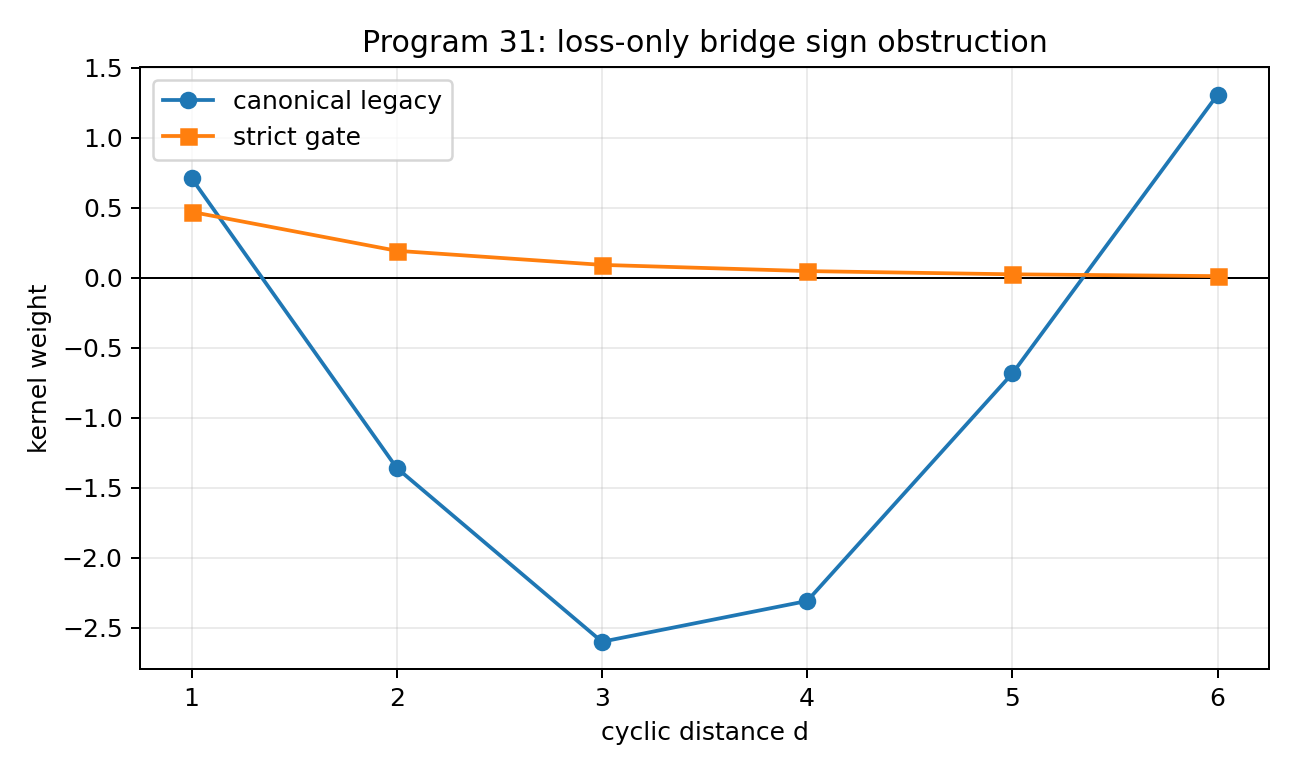
\includegraphics[width=0.82\textwidth]{FIN_Programs_31_40_Figures/program31_loss_bridge.png}
\caption{Canonical legacy and strict radial rows. Positive attenuation preserves signs and therefore cannot supply the missing phase transformation.}
\end{figure}

For \(c>0\), four signs disagree. For \(c<0\), the signs at \(d=1,6\) disagree. Allowing \(r_d=0\) cannot produce the nonzero strict target at a mismatched distance. Therefore no loss-only diagonal multiplier exists. \textbf{\statusProven{}}

Even with an independently chosen retention for every distance, the positive-normalization residual is bounded below by

\[
0.219167,
\]

or (42.25\%) of the strict-row norm.

\section{Additive Loewner test}

An alternative passive-loss proposal is

\[
A_s=A_\ell+B,
\qquad B\succeq0.
\]

On \(C_{12}\), the computed difference satisfies

\[
\lambda(B)\subset
[8.9\times10^{-16},22.9541],
\]

with rank eleven. On a twelve-point interval obtained by extrapolating the same analytic formulas to \(|i-j|\le11\),

\[
\lambda(B)\subset[-4.69964,20.1323].
\]

Thus the additive dissipative interpretation works on the declared cycle realization but is not support-independent. \textbf{[Strong numerical evidence]}

\section{Verdict}

\begin{itemize}
\item 
Complete bridge by positive attenuation alone: \textbf{\statusRefuted{}}.

\item 
Passive additive correction on \(C_{12}\): \textbf{\statusStrong{}}.

\item 
Geometry-independent completion theorem: \textbf{[Refuted by the interval counterexample]}.

\item 
Required additional ingredient: a phase/\allowbreak{}frequency transformation or non-diagonal distance-mixing map. \textbf{\statusProven{}}

\end{itemize}

\par\medskip\hrule\medskip

\chapter{Part III — Program 32: Markov admissibility of the legacy kernel}

\section{Question}

Does the canonical signed legacy kernel itself generate classical information loss?

\section{Candidate generator}

Define the circulant zero-diagonal matrix \(W_\ell\) on \(C_{12}\) and

\[
A_\ell=\operatorname{diag}(W_\ell\mathbf1)-W_\ell.
\]

A continuous-time Markov generator \(-A_\ell\) requires nonnegative off-diagonal transition rates, equivalently \((W_\ell)_{xy}\ge0\) for \(x\ne y\).

\section{Failure of the raw signed row}

The row sum is

\[
s_\ell=-11.174051962,
\]

and

\[
\sigma(A_\ell)\subset[-21.377059810,0].
\]

\begin{figure}[htbp]
\centering
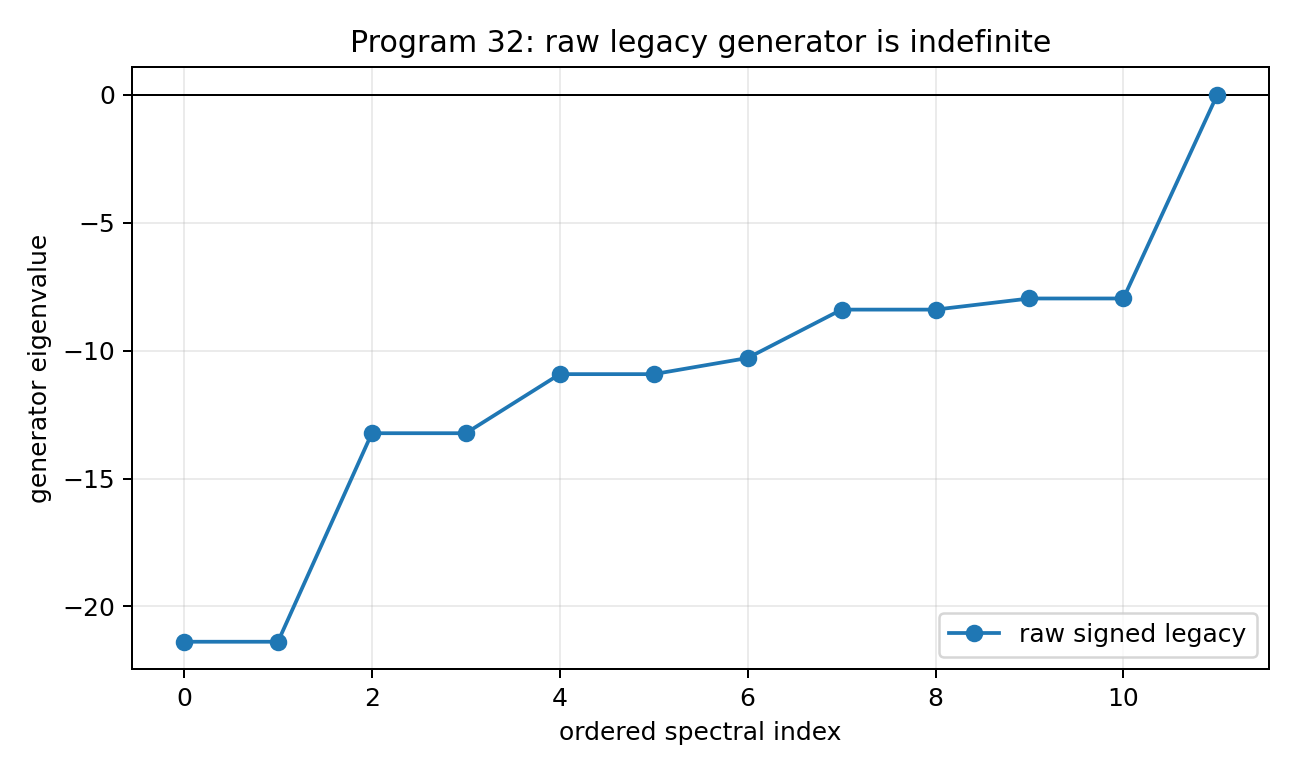
\includegraphics[width=0.82\textwidth]{FIN_Programs_31_40_Figures/program32_legacy_spectrum.png}
\caption{Spectrum of the raw signed legacy Laplacian candidate on the twelve-cycle. Eleven nonconstant eigenvalues are negative.}
\end{figure}

The matrix exponential already violates positivity at short time:

\begin{center}
\begingroup\small
\setlength{\tabcolsep}{3.5pt}
\renewcommand{\arraystretch}{1.16}
\begin{longtable}{@{}p{0.204\textwidth}p{0.339\textwidth}p{0.317\textwidth}@{}}
\toprule
\textbf{\(t\)} & \textbf{\(min e^{-tA_\ell}\)} & \textbf{\(|e^{-tA_\ell}|_2\)} \\
\midrule
\endhead
\(0.001\) & \(-0.00263292\) & \(1.02161\) \\
\(0.01\) & \(-0.0295213\) & \(1.23834\) \\
\(0.1\) & \(-1.06641\) & \(8.47996\) \\
\bottomrule
\end{longtable}
\endgroup
\end{center}

The raw legacy row is not a stochastic information-loss generator. \textbf{\statusProven{}}

\section{Nonunique positivity repairs}

Two elementary replacements are

\[
W_\ell^+=\max(W_\ell,0),
\qquad
W_\ell^{|\cdot|}=|W_\ell|.
\]

Both yield symmetric Markov semigroups, but:

\begin{center}
\begingroup\small
\setlength{\tabcolsep}{3.5pt}
\renewcommand{\arraystretch}{1.16}
\begin{longtable}{@{}p{0.190\textwidth}p{0.346\textwidth}p{0.324\textwidth}@{}}
\toprule
\textbf{Repair} & \textbf{Spectral gap} & \textbf{\(\mathcal{I}(P_1\delta_0)\)} \\
\midrule
\endhead
positive part & \(0.710493827\) & \(0.261871502\) \\
absolute value & \(15.185443105\) & \(7.73\times10^{-14}\) \\
\bottomrule
\end{longtable}
\endgroup
\end{center}

The gap ratio is \(21.3731\). The same static signed row therefore admits radically different loss dynamics after equally elementary nonlinear repairs. \textbf{\statusProven{}}

\section{Verdict}

\begin{itemize}
\item 
Raw legacy kernel as a Markov loss law: \textbf{\statusRefuted{}}.

\item 
Existence of repaired Markov laws: \textbf{\statusProven{}}.

\item 
Unique repair selected by the legacy formula: \textbf{\statusRefuted{}}.

\item 
A microscopic or operational repair criterion remains necessary.

\end{itemize}

\par\medskip\hrule\medskip

\chapter{Part IV — Program 33: hazard reconstruction of nonlinear strict damping}

\section{Envelope-only question}

After explicitly setting the phase obstruction aside, can the denominator change be written as cumulative negative feedback?

Define

\[
E_\ell(d)=\frac1{1+0.01d},
\qquad
E_s(d)=\frac1{1+d^{1.8}},
\]

and

\[
R_d=\frac{E_s(d)}{E_\ell(d)}
=\frac{1+0.01d}{1+d^{1.8}}.
\]

\section{Discrete hazard}

Write

\[
R_d=\prod_{j=1}^{d}\rho_j,
\qquad
h_j=-\log\rho_j
=\log\frac{R_{j-1}}{R_j},
\qquad R_0=1.
\]

All twelve hazards are positive. Selected values are:

\begin{center}
\begingroup\small
\setlength{\tabcolsep}{3.5pt}
\renewcommand{\arraystretch}{1.16}
\begin{longtable}{@{}p{0.143\textwidth}p{0.373\textwidth}p{0.344\textwidth}@{}}
\toprule
\textbf{\(d\)} & \textbf{\(R_d\)} & \textbf{\(h_d\)} \\
\midrule
\endhead
1 & \(0.505000\) & \(0.683197\) \\
2 & \(0.227567\) & \(0.797115\) \\
3 & \(0.125233\) & \(0.597268\) \\
6 & \(0.0405233\) & \(0.303959\) \\
12 & \(0.0126404\) & \(0.145740\) \\
\bottomrule
\end{longtable}
\endgroup
\end{center}

\begin{figure}[htbp]
\centering
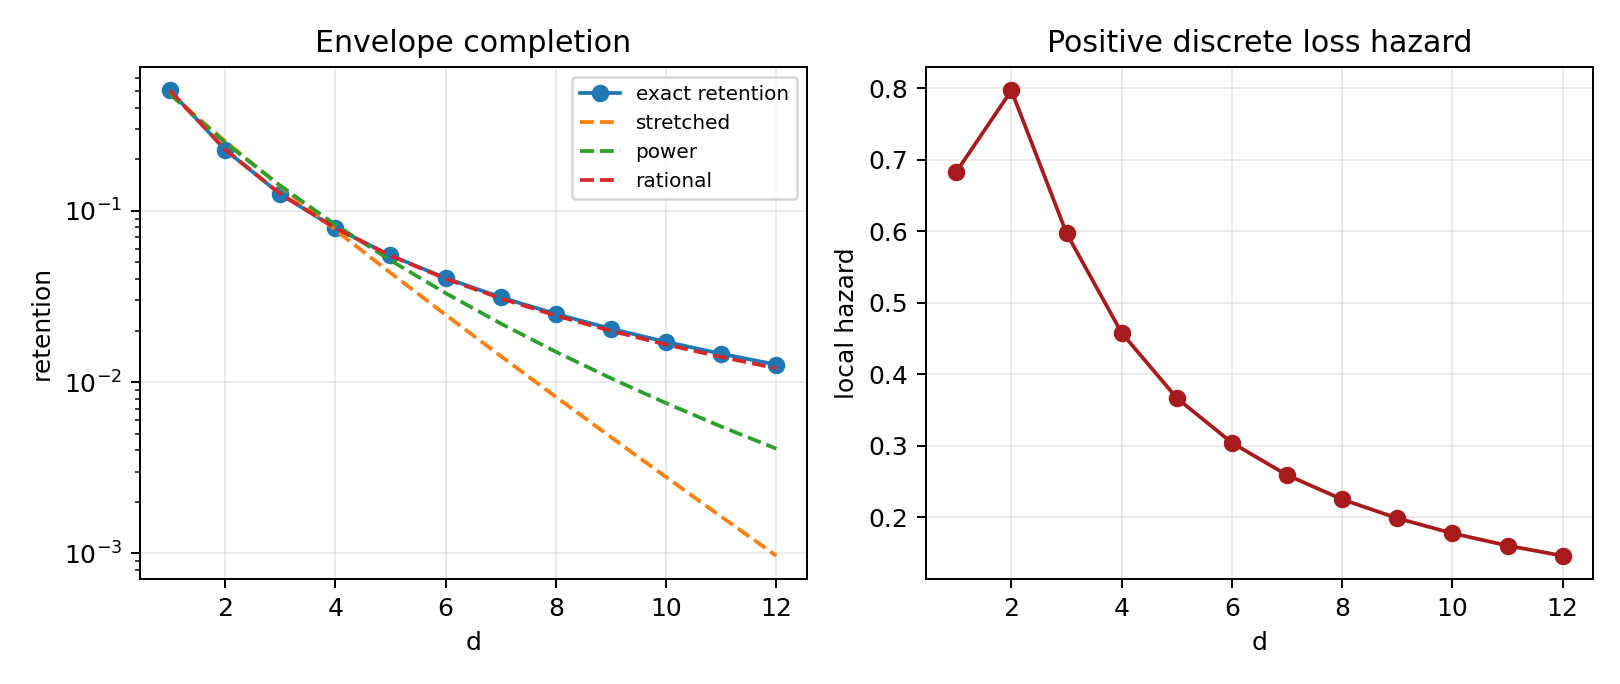
\includegraphics[width=0.82\textwidth]{FIN_Programs_31_40_Figures/program33_hazard.png}
\caption{Exact legacy-to-strict envelope retention, fitted candidate laws, and the positive discrete hazard sequence.}
\end{figure}

Hence an exact cumulative-loss representation exists for the envelopes. \textbf{\statusProven{}}

\section{Competing feedback laws}

Four two-parameter or simpler families were fitted without inserting the exact numerator:

\begin{center}
\begingroup\small
\setlength{\tabcolsep}{3.5pt}
\renewcommand{\arraystretch}{1.16}
\begin{longtable}{@{}p{0.192\textwidth}p{0.328\textwidth}p{0.182\textwidth}p{0.158\textwidth}@{}}
\toprule
\textbf{Law} & \textbf{Best parameters} & \textbf{Relative \(L^2\) error} & \textbf{Maximum relative error} \\
\midrule
\endhead
\(e^{-\gamma d}\) & \(\gamma=0.687293\) & \(0.10797\) & \(0.9793\) \\
\(e^{-\gamma d^q}\) & \(\gamma=0.727191,q=0.907984\) & \(0.09705\) & \(0.9236\) \\
\((1+cd)^{-p}\) & \(c=0.142184,p=5.52676\) & \(0.07769\) & \(0.6774\) \\
\((1+bd^\eta)^{-1}\) & \(b=0.982316,\eta=1.78137\) & \(0.003233\) & \(0.0487\) \\
\bottomrule
\end{longtable}
\endgroup
\end{center}

Under (1\%) multiplicative perturbations, the rational-fit (95\%) interval was approximately

\[
\eta\in[1.7506,1.8125].
\]

This supports the numerical robustness of the exponent within the declared finite family. It does not source the exponent. \textbf{\statusStrong{}}

\section{Nonuniqueness theorem}

Every strictly decreasing positive sequence admits a unique discrete hazard sequence. The same hazard can be implemented by erasure, dephasing, hidden-state mixing, environmental leakage, absorption, or feedback. Therefore the hazard representation does not identify a microscopic mechanism. \textbf{\statusProven{}}

\section{Verdict}

\begin{itemize}
\item 
Positive envelope-loss representation: \textbf{\statusProven{}}.

\item 
Unique microscopic negative coupling: \textbf{\statusRefuted{}}.

\item 
Derivation of \(\eta=1.8\) from information theory: \textbf{[Not established]}.

\item 
Phase completion: \textbf{still absent by Program 31}.

\end{itemize}

\par\medskip\hrule\medskip

\chapter{Part V — Program 34: stability cone of negative feedback}

\section{Two placements of feedback}

Using the positive strict weights \(w_d\), compare

\[
w_d^{\exp}(\gamma)=w_de^{-\gamma d}
\]

with

\[
w_d^{\rm lin}(\gamma)=w_d(1-\gamma d).
\]

Both express decreasing coupling, but only the first is automatically positive.

\section{Exact admissibility boundary}

Because \(w_d>0\) for \(d=1,\ldots,6\), the linear law has nonnegative rates precisely when

\[
0\le\gamma\le\frac1{d_{\max}}=\frac16.
\]

Beyond this value, at least one off-diagonal transition rate is negative. \textbf{\statusProven{}}

\begin{figure}[htbp]
\centering
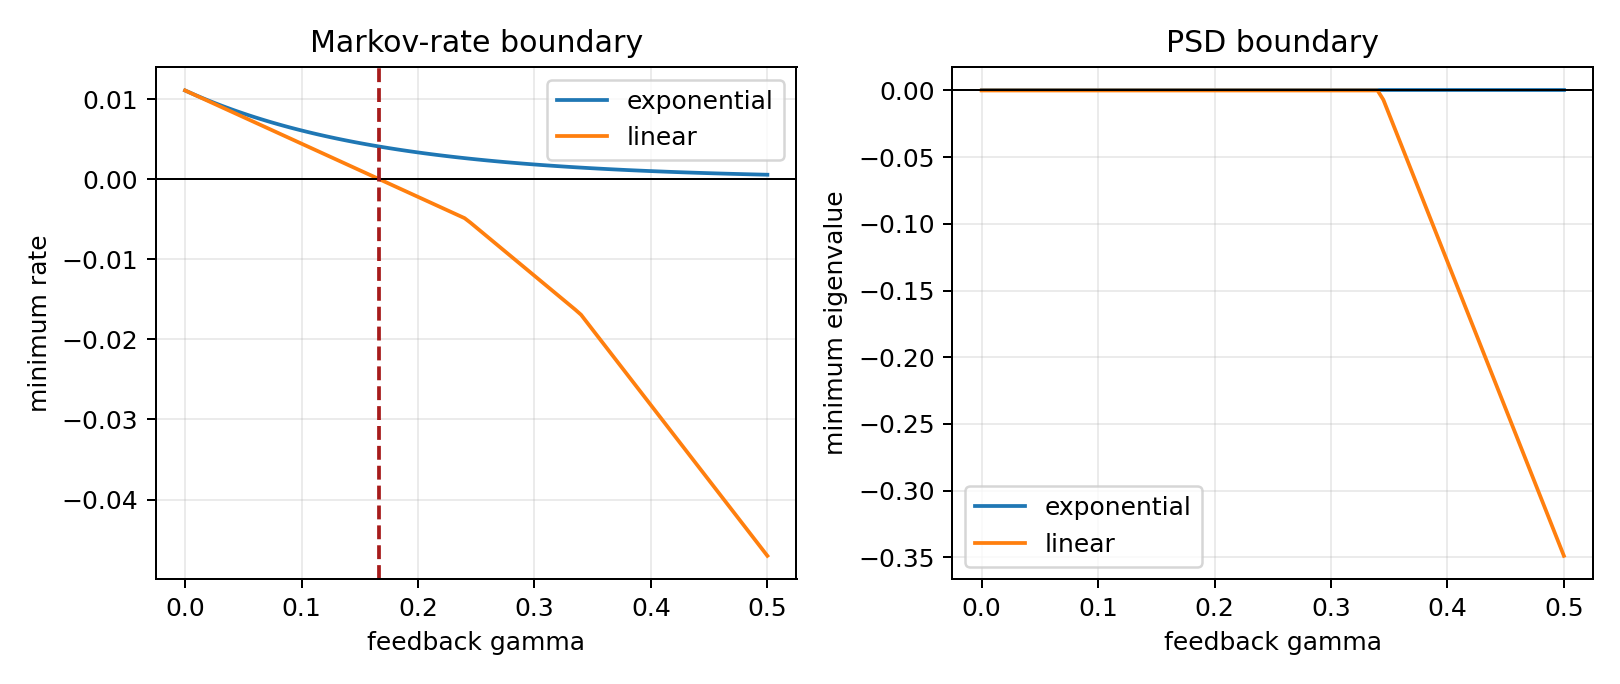
\includegraphics[width=0.82\textwidth]{FIN_Programs_31_40_Figures/program34_stability_cone.png}
\caption{Markov-rate and spectral boundaries for exponential retention and linear subtraction.}
\end{figure}

Selected results are:

\begin{center}
\begingroup\footnotesize
\setlength{\tabcolsep}{3.5pt}
\renewcommand{\arraystretch}{1.16}
\begin{longtable}{@{}p{0.161\textwidth}p{0.103\textwidth}p{0.220\textwidth}p{0.200\textwidth}p{0.176\textwidth}@{}}
\toprule
\textbf{Law} & \textbf{\(\gamma\)} & \textbf{Minimum weight} & \textbf{Minimum eigenvalue} & \textbf{Gap} \\
\midrule
\endhead
exponential & \(0.4\) & \(+0.00100432\) & numerical zero & \(0.268463\) \\
linear & \(1/6\) & \(0\) & numerical zero & \(0.386440\) \\
linear & \(0.2\) & \(-0.00221416\) & numerical zero & \(0.312904\) \\
linear & \(0.4\) & \(-0.0282175\) & \(-0.128313\) & — \\
\bottomrule
\end{longtable}
\endgroup
\end{center}

At \(\gamma=0.2\),

\[
\min e^{-0.001A_\gamma}=-2.21\times10^{-6},
\]

so Markov positivity fails immediately even though the quadratic form has not yet become negative. At \(\gamma=0.4\), both rate and spectral conditions fail.

One hundred random-distribution tests found no relative-information increase for exponential \(\gamma=0.4\) or boundary-linear \(\gamma=1/6\). \textbf{[Strong numerical evidence consistent with data processing]}

\section{Verdict}

\begin{itemize}
\item 
Exponential retention: \textbf{[Proven Markov-admissible]}.

\item 
Unrestricted linear subtraction: \textbf{\statusRefuted{}}.

\item 
Positive semidefiniteness alone as a stochastic criterion: \textbf{\statusRefuted{}}.

\item 
Physical choice of \(\gamma\): \textbf{not supplied}.

\end{itemize}

\par\medskip\hrule\medskip

\chapter{Part VI — Program 35: information destruction versus environmental transfer}

\section{Declared channel and dilation}

For the strict stochastic semigroup \(P_t=e^{-tA_s}\), define the measure-and-prepare channel

\[
\Phi_t(\rho)
=\sum_{x,y}P_t(y|x)
\langle x|\rho|x\rangle
|y\rangle\langle y|.
\]

It has the isometry

\[
V_t|x\rangle
=\sum_y\sqrt{P_t(y|x)}
|y\rangle_S|x,y\rangle_E.
\]

The finite computation gives

\[
\|V_t^\dagger V_t-I\|_F=1.06\times10^{-15}
\]

and a reduced-channel residual \(1.39\times10^{-16}\). This is a direct instance of \href{https://doi.org/10.1090/S0002-9939-1955-0069403-4}{Stinespring dilation}. \textbf{\statusProven{}}

\section{Information ledger}

Starting from \(\delta_0\), at \(t=1\):

\[
H(p_1)=2.225996234,
\qquad
D(p_1\|u)=0.258910416,
\]

\[
\operatorname{Tr}\rho_S^2=0.135124653.
\]

For the pure dilation,

\[
S(SE)=0,
\qquad
S(S)=S(E)=2.225996234,
\]

and

\[
I(S:E)=4.451992468.
\]

\begin{figure}[htbp]
\centering
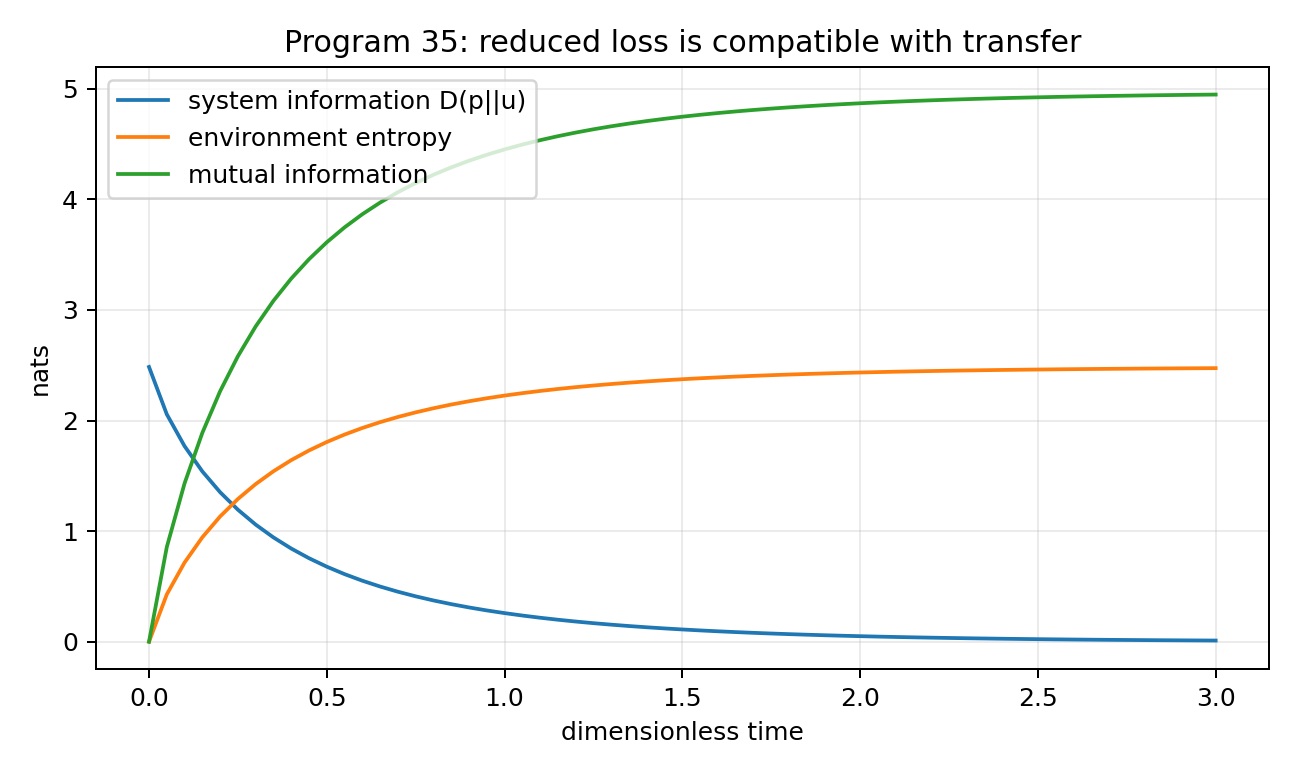
\includegraphics[width=0.82\textwidth]{FIN_Programs_31_40_Figures/program35_information_ledger.png}
\caption{Reduced-system information, environment entropy, and mutual information for the explicit isometric dilation.}
\end{figure}

The reduced system loses accessible information while the joint description remains pure. This is compatible with the general principle that reduced open-system loss need not be fundamental deletion. \textbf{\statusProven{}}

\section{Identifiability obstruction}

Every finite completely positive trace-preserving channel admits an isometric dilation. Therefore system-only observations cannot decide whether their reduced loss is fundamental or environmental. One needs environment access, recovery operations, or an additional axiom declaring the system closed. \textbf{\statusProven{}}

The \href{https://doi.org/10.1103/PhysRevLett.98.080502}{no-hiding theorem} further constrains where quantum information can reside in a unitary embedding, but the present result needs only Stinespring dilation.

\section{Verdict}

\begin{itemize}
\item 
Reduced-system information loss: \textbf{\statusProven{}}.

\item 
Compatibility with transfer and correlation: \textbf{\statusProven{}}.

\item 
Fundamental destruction inferred from system data: \textbf{[Refuted as an inference]}.

\item 
Thermodynamic heat cost: \textbf{not derived}.

\end{itemize}

\par\medskip\hrule\medskip

\chapter{Part VII — Program 36: open-system coupling-sign gauge}

\section{Model}

Let

\[
B=\frac{A_s-A_\ell}{\|A_s-A_\ell\|_F}
\]

on the declared cycle and define

\[
H_{\rm tot}(g)
=A_s\otimes I_E
+I_S\otimes H_E
+gB\otimes X_E.
\]

The numerical study used a two-level environment,

\[
H_E=0.7\sigma_z,
\qquad X_E=\sigma_x,
\qquad |g|=0.8.
\]

\section{Exact parity theorem}

Suppose a bath parity \(P_E\) satisfies

\[
P_EH_EP_E=H_E,
\qquad
P_EX_EP_E=-X_E,
\qquad
P_E\tau_EP_E=\tau_E.
\]

Then

\[
H_{\rm tot}(-g)
=(I\otimes P_E)H_{\rm tot}(g)(I\otimes P_E),
\]

and, after tracing out the bath,

\[
\Phi_t^{(-g)}=\Phi_t^{(g)}.
\]

Thus the system cannot identify the sign. \textbf{\statusProven{}}

\section{Numerical sign tests}

Across three system probes and 41 times:

\[
\max_t D\!\left(\Phi_t^{(+g)},\Phi_t^{(-g)}\right)=0
\]

for the symmetric bath.

For a bath polarized along \(\sigma_x\), the maximum system trace distance became

\[
0.0468978.
\]

A calibrated odd environment record reached a difference

\[
0.368994.
\]

\begin{figure}[htbp]
\centering
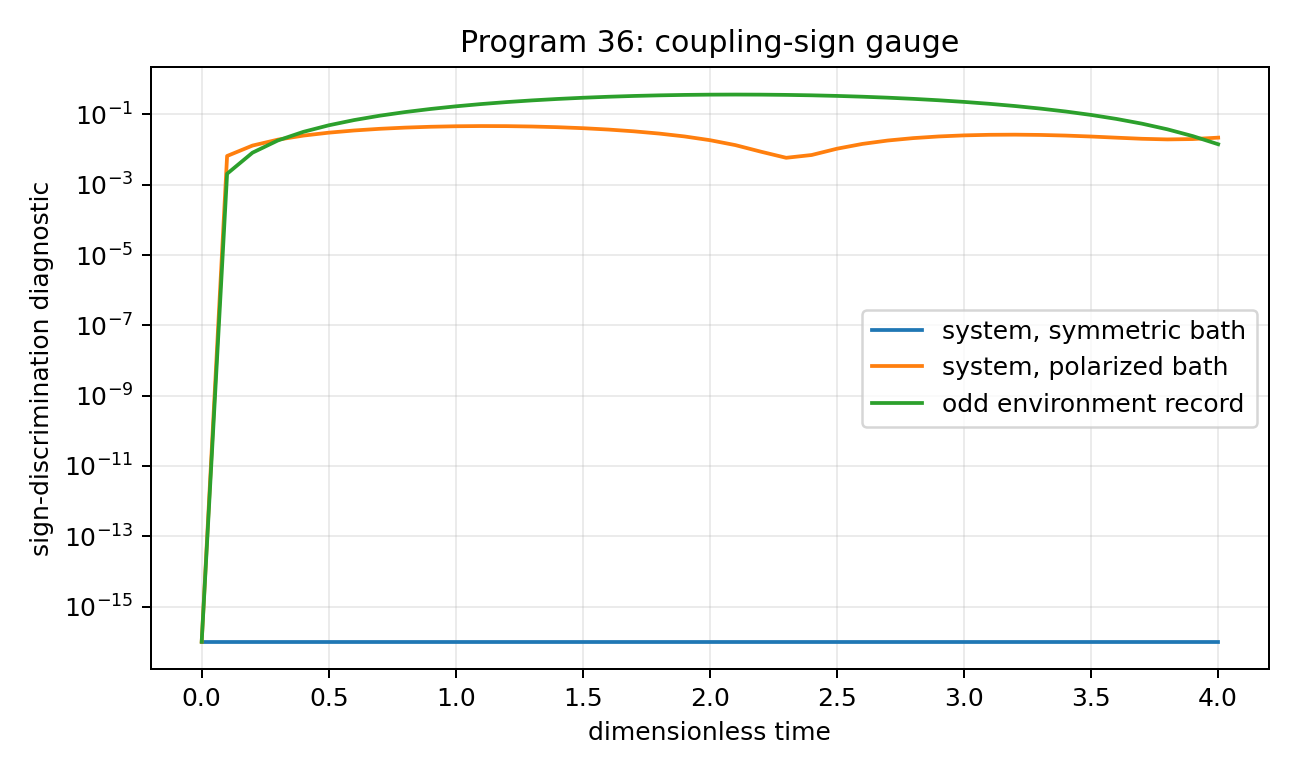
\includegraphics[width=0.82\textwidth]{FIN_Programs_31_40_Figures/program36_sign_gauge.png}
\caption{System and environment sign-discrimination diagnostics. Symmetric-bath system dynamics is exactly sign blind.}
\end{figure}

The transformation

\[
(g,X_E)\longmapsto(-g,-X_E)
\]

is a sign gauge. A statement that \(g<0\) has operational content only after the polarity of \(X_E\) is fixed independently. \textbf{\statusProven{}}

\section{Verdict}

\begin{itemize}
\item 
System-only coupling sign in a parity-symmetric environment: \textbf{[Unidentifiable]}.

\item 
Sign after a calibrated odd reference: \textbf{[Identifiable in the declared model]}.

\item 
Internal FIN source of that reference: \textbf{[Not established]}.

\item 
Selector closure from coupling sign: \textbf{[Not obtained]}.

\end{itemize}

\par\medskip\hrule\medskip

\chapter{Part VIII — Program 37: feedback and entropy-production ledger}

\section{Positive-rate feedback law}

Let \(b_i=\cos(2\pi i/12)\). Starting from the strict positive rates, define

\[
w_{ij}(\theta)
=w^s_{ij}
\exp\!\left[-\frac\theta2(b_i-b_j)\right].
\]

These rates satisfy detailed balance with

\[
\pi_i(\theta)\propto e^{-\theta b_i}.
\]

The controller used

\[
\dot\theta=-0.8\theta,
\qquad \theta(0)=1.4.
\]

The quadratic controller loss fell from \(0.98\) to \(6.64\times10^{-5}\). The instantaneous Markov entropy-production rate

\[
\sigma
=\sum_{i<j}
(w_{ij}p_j-w_{ji}p_i)
\log\frac{w_{ij}p_j}{w_{ji}p_i}
\]

remained nonnegative to numerical precision. \textbf{[Strong evidence; nonnegativity follows termwise]}

\section{Stable does not imply variational}

Consider the stable two-coordinate controller

\[
\dot\theta=J\theta,
\qquad
J=
\begin{pmatrix}
-0.8&1.7\\
-1.7&-0.8
\end{pmatrix}.
\]

Its eigenvalues are

\[
-0.8\pm1.7i,
\]

so it is asymptotically stable. However,

\[
\frac{\|J-J^T\|_F}{\|J\|_F}=1.80964,
\]

and the work around the unit circle is

\[
\oint F\cdot d\theta=-10.6814\ne0.
\]

No scalar potential generates this feedback in the declared Euclidean coordinates. \textbf{\statusProven{}}

\section{Thermodynamic accounting boundary}

Feedback thermodynamics requires measurement records, controller memory, work, and mutual-information terms, as made explicit by the \href{https://doi.org/10.1103/PhysRevLett.104.090602}{Sagawa–Ueda feedback relation}. A decreasing system functional alone is not a complete entropy ledger.

\section{Verdict}

\begin{itemize}
\item 
Stable negative feedback: \textbf{[Constructed]}.

\item 
Compatibility with nonnegative Markov entropy production: \textbf{[Proven for the model]}.

\item 
Automatic existence of an action: \textbf{\statusRefuted{}}.

\item 
Kernel-derived controller, target, or polarity: \textbf{[Not established]}.

\end{itemize}

\par\medskip\hrule\medskip

\chapter{Part IX — Program 38: wave–diffusion observer test}

\section{Common positive feedback family}

Define

\[
w_d(g)=w_d^s e^{gd/6},
\qquad
A(g)=D(g)-W(g).
\]

The same signed parameter appears in

\[
U_t(g)=e^{-itA(g)}
\]

and

\[
P_t(g)=e^{-tA(g)}.
\]

No positivity problem arises for finite \(g\).

\section{Short-time theorem}

For a localized preparation \(|x\rangle\),

\[
P_t(x|x)=1-A_{xx}t+O(t^2),
\]

whereas

\[
|U_t(x|x)|^2
=1-\operatorname{Var}_x(A)t^2+O(t^4).
\]

The fitted escape exponents were:

\begin{center}
\begingroup\small
\setlength{\tabcolsep}{3.5pt}
\renewcommand{\arraystretch}{1.16}
\begin{longtable}{@{}p{0.228\textwidth}p{0.314\textwidth}p{0.318\textwidth}@{}}
\toprule
\textbf{\(g\)} & \textbf{diffusion} & \textbf{unitary wave} \\
\midrule
\endhead
\(-0.5\) & \(0.99907\) & \(2.00000\) \\
\(0\) & \(0.99895\) & \(2.00000\) \\
\(+0.5\) & \(0.99879\) & \(2.00000\) \\
\bottomrule
\end{longtable}
\endgroup
\end{center}

No clock rescaling changes a generic linear leading term into a quadratic one. \textbf{\statusProven{}}

\section{Chapman–Kolmogorov and phase records}

For diffusion,

\[
P_{2t}=P_t^2
\]

to residuals below \(4\times10^{-15}\).

For unitary population matrices

\[
M_t(y|x)=|U_t(y,x)|^2,
\]

the Chapman–Kolmogorov residual reached \(0.93\), because unobserved amplitudes interfere.

For the double-path input

\[
|\psi_\varphi\rangle
=\frac{|0\rangle+e^{i\varphi}|3\rangle}{\sqrt2},
\]

the best-detector visibility remained between \(0.966\) and \(0.9995\) over the tested \(g\)-values.

\begin{figure}[htbp]
\centering
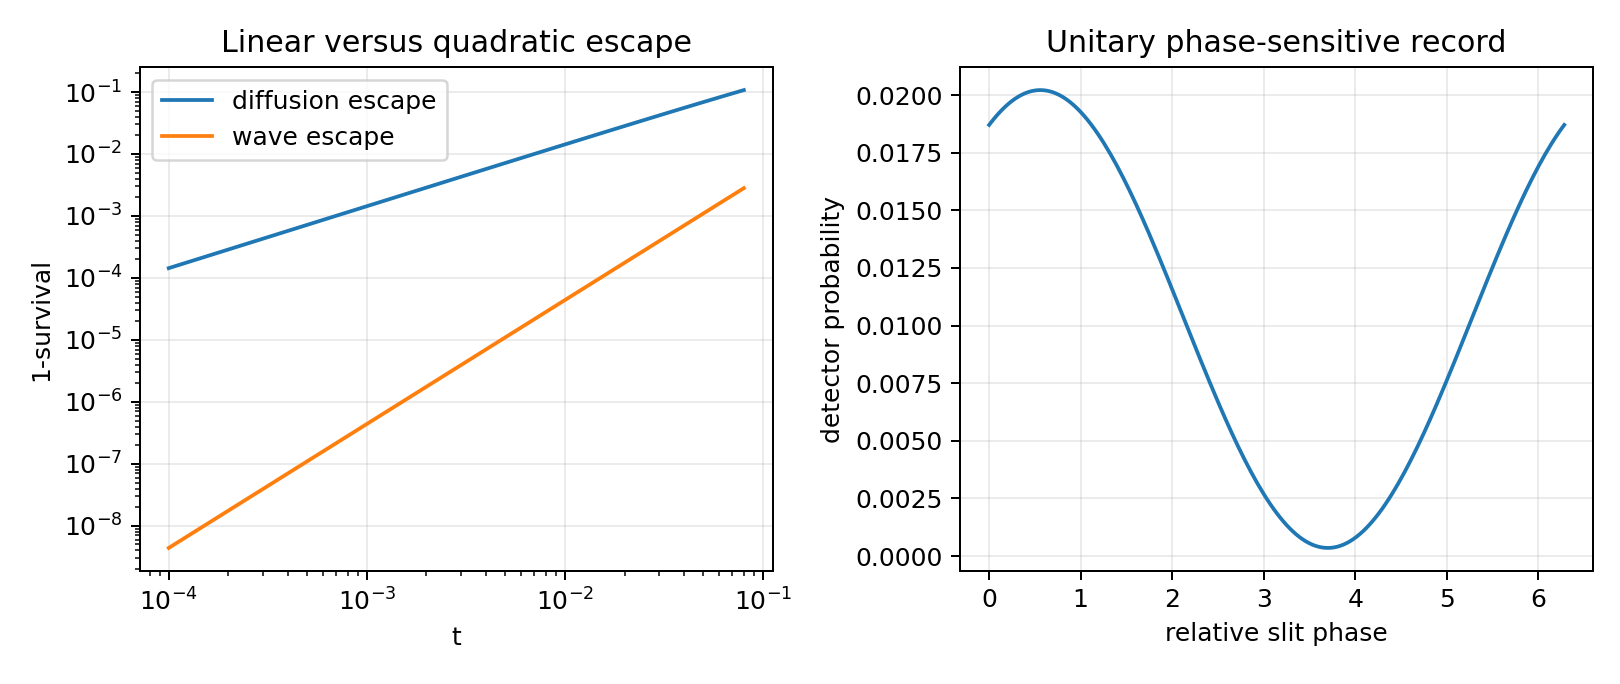
\includegraphics[width=0.82\textwidth]{FIN_Programs_31_40_Figures/program38_wave_diffusion.png}
\caption{Linear diffusive versus quadratic unitary escape and a phase-sensitive double-path record.}
\end{figure}

Intermediate interventions and phase variation therefore distinguish the temporal categories without invoking an undefined observer collapse. This is consistent with the operational process-tensor approach of \href{https://doi.org/10.1103/PhysRevLett.120.040405}{Pollock et al.}.

\section{Verdict}

\begin{itemize}
\item 
Common spatial feedback parameter: \textbf{[Constructed]}.

\item 
Selection of wave versus diffusion by its sign: \textbf{\statusRefuted{}}.

\item 
Operational distinction by early time, interventions, or phase: \textbf{\statusProven{}}.

\item 
Physical clock or observer ontology: \textbf{[Not derived]}.

\end{itemize}

\par\medskip\hrule\medskip

\chapter{Part X — Program 39: structural identifiability of sign and scale}

\section{Gauge-blind observation model}

The finite identification model uses Poisson means

\[
\lambda_r
=\lambda_0+\epsilon
+E_r\bigl[\tau(gb_r+hc_r)\bigr]^2,
\]

where g is the signed coupling, tau is clock scale, epsilon is background, and h c\_r is an optional calibrated reference.

Without the reference h=0, only the product tau g is observed and the likelihood is symmetric under sign reversal.

\section{Fisher-rank test}

For the declared true point

\[
(g,\tau,\epsilon)=(-0.42,1.06,1.3),
\]

the no-reference Fisher eigenvalues were

\[
(1.54\times10^{-14},0.2310,417.626),
\]

so the rank was two.

With a calibrated reference they became

\[
(0.1078,113.666,615.176),
\]

and the rank became three. \textbf{[Strong numerical evidence]}

\begin{figure}[htbp]
\centering
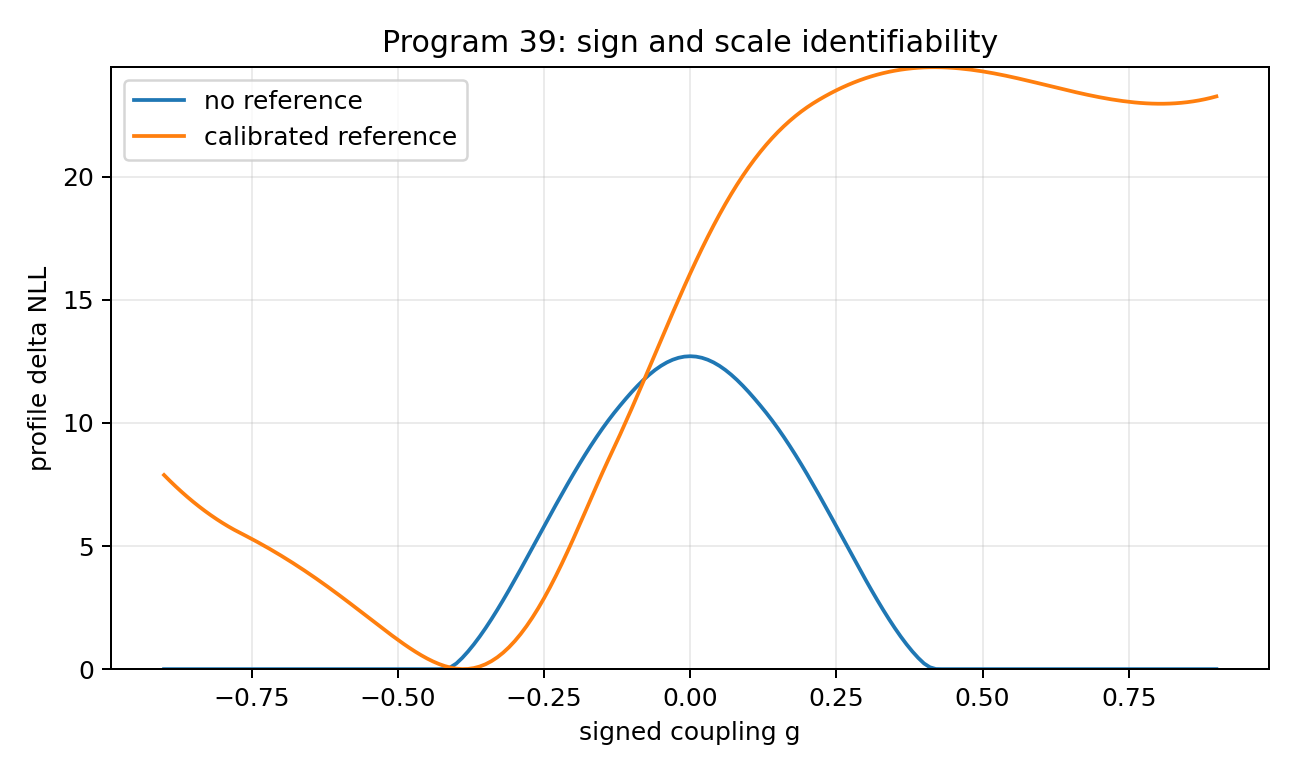
\includegraphics[width=0.82\textwidth]{FIN_Programs_31_40_Figures/program39_identifiability.png}
\caption{Profile likelihood for the signed coupling with and without a calibrated reference channel.}
\end{figure}

The no-reference sign difference in profile negative log likelihood was exactly zero. With the reference it was

\[
\Delta\mathrm{NLL}=24.3252
\]

at the true magnitude. The fitted sign was \(g=-0.39\). Reversing apparatus polarity without relational recoding changed the fit to \(g=+0.39\).

\section{Identifiability theorem for the declared family}

The transformations

\[
(g,B)\sim(cg,B/c),
\qquad
(A,\tau)\sim(cA,\tau/c),
\qquad
(g,X_E)\sim(-g,-X_E)
\]

are observational equivalences unless an amplitude, clock, and polarity reference is supplied. A nonzero signed coupling is not an invariant of uncalibrated data. \textbf{\statusProven{}}

\section{Verdict}

\begin{itemize}
\item 
Sign without reference: \textbf{[Globally unidentifiable]}.

\item 
Sign with independently calibrated interference: \textbf{[Identifiable in the model]}.

\item 
Strict internal source of clock, amplitude, and polarity: \textbf{[Absent]}.

\item 
A prior preference for \(g<0\) as evidence: \textbf{[Rejected]}.

\end{itemize}

\par\medskip\hrule\medskip

\chapter{Part XI — Program 40: blinded negative-coupling challenge}

\section{Frozen synthetic protocol}

Four models were declared before generating the counts:

\begin{itemize}
\item 
negative operational coupling, \(g=-0.28\), with a correlated odd environment record;

\item 
zero coupling;

\item 
positive operational coupling, \(g=+0.28\);

\item 
a static mimic with the same system operator as the negative model but no correlated environment record.

\end{itemize}

Training used diffusion at \(t=0.35\), unitary populations at \(t=0.55\), and one environment record. Held-out data used diffusion at \(t=1.05\), unitary populations at \(t=1.35\), a double-path record at \(t=1.8\), and two environment records. Clock and SPAM nuisance parameters were fitted on training data only.

The protocol commitment was

\begin{Verbatim}[fontsize=\small]
1778a5f93f824bc09a4948c9124b28bb23e823b950970a1b01c51aa3bcd1903b
\end{Verbatim}

This is a deterministic internal commitment, not an externally timestamped preregistration.

\section{Results}

With 500 shots per block and 60 trials per model, the confusion matrix was

\[
\begin{pmatrix}
56&4&0&0\\
0&49&1&10\\
0&1&58&1\\
0&18&0&42
\end{pmatrix},
\]

in the order negative, zero, positive, static mimic.

\begin{figure}[htbp]
\centering
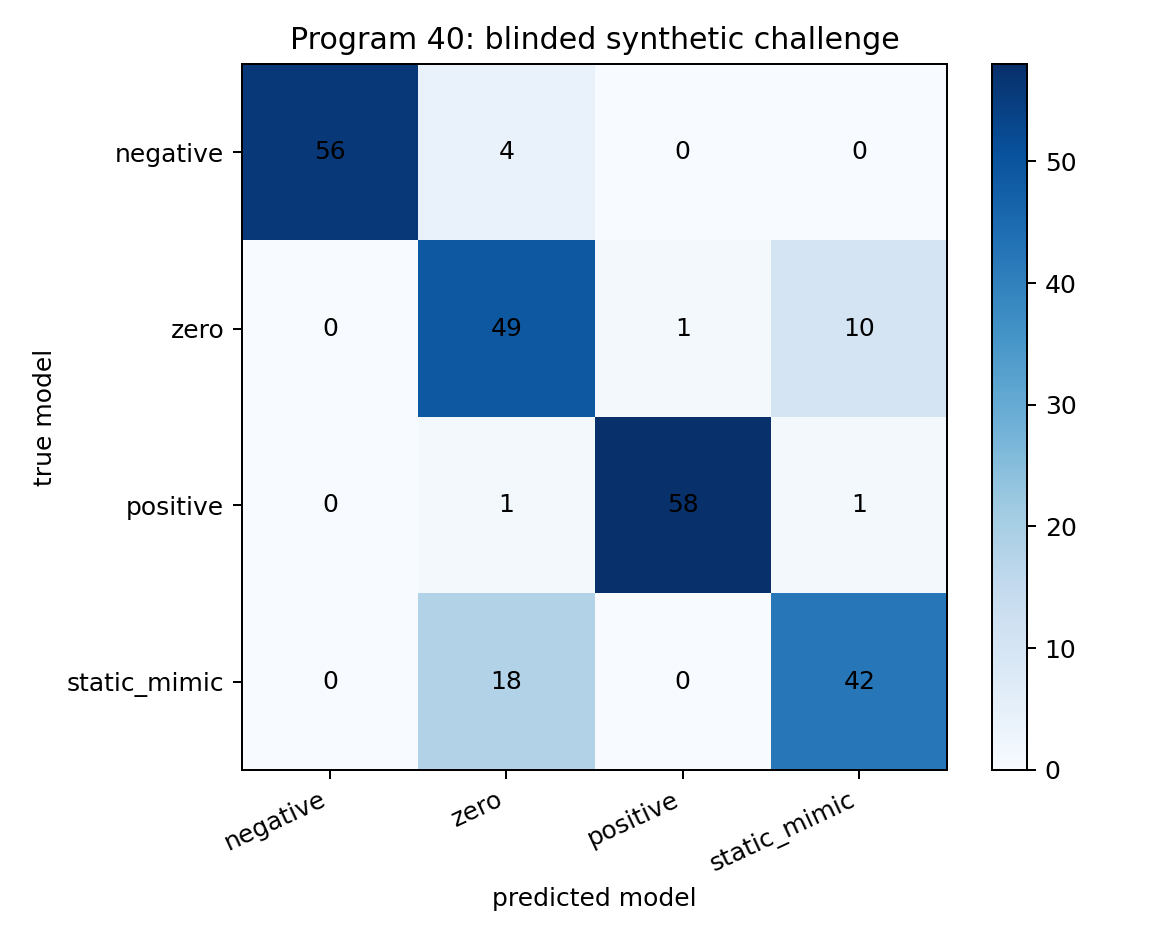
\includegraphics[width=0.82\textwidth]{FIN_Programs_31_40_Figures/program40_confusion.png}
\caption{Confusion matrix for the four-model blinded synthetic held-out challenge.}
\end{figure}

Overall accuracy was

\[
0.85417.
\]

Per-model accuracies were:

\begin{center}
\begingroup\small
\setlength{\tabcolsep}{3.5pt}
\renewcommand{\arraystretch}{1.16}
\begin{longtable}{@{}p{0.420\textwidth}p{0.420\textwidth}@{}}
\toprule
\textbf{Model} & \textbf{Accuracy} \\
\midrule
\endhead
negative & \(0.9333\) \\
zero & \(0.8167\) \\
positive & \(0.9667\) \\
static mimic & \(0.7000\) \\
\bottomrule
\end{longtable}
\endgroup
\end{center}

The median winning held-out log-likelihood margin was \(5.49464\).

\section{Causal nonidentifiability result}

After removing environment records, the negative operational model and the static mimic had system-signature residual

\[
0.
\]

They are exactly the same system process by construction. No amount of additional system-only data can distinguish “dynamical negative coupling” from “the same static operator” in this candidate pair. The environment record, intervention on the coupling, or a different-size prediction is essential. \textbf{\statusProven{}}

\section{Verdict}

\begin{itemize}
\item 
Synthetic pipeline sensitivity to the negative model: \textbf{\statusStrong{}}.

\item 
Unique causal identification from system dynamics: \textbf{\statusRefuted{}}.

\item 
Hardware validation: \textbf{[Not executed]}.

\item 
Strict legacy-to-strict source theorem: \textbf{[Not obtained]}.

\item 
Evidence for fundamental physics: \textbf{none}.

\end{itemize}

\par\medskip\hrule\medskip

\chapter{Part XII — Can negative information coupling be placed in an action?}

\section{Static quadratic correction}

On \(C_{12}\), the positive difference \(B=A_s-A_\ell\succeq0\) permits the Euclidean quadratic correction

\[
S_s[\phi]
=S_\ell[\phi]
+\frac12\phi^TB\phi.
\]

This stabilizes a static precision form. It does not prove temporal dissipation or information loss: the same positive operator can enter either \(e^{-itA}\) or \(e^{-tA}\). \textbf{\statusProven{}}

\section{Why an ordinary potential is insufficient}

A conservative action

\[
S[q]=\int L(q,\dot q)\,dt
\]

does not by itself encode irreversible loss. Classical damping may be represented conditionally by a Rayleigh function

\[
\frac{d}{dt}\frac{\partial L}{\partial\dot q}
-\frac{\partial L}{\partial q}
+\frac{\partial\mathcal R}{\partial\dot q}=0,
\]

or statistically by an \href{https://doi.org/10.1103/PhysRev.91.1505}{Onsager–Machlup functional}. These are additional dynamical structures.

Program 37 gives an explicit stable feedback field with nonzero circulation. It cannot be obtained as the gradient of a scalar potential in the declared coordinates. A post-hoc (V(K)) therefore does not solve the operational loss problem.

\section{Minimal closed-system action with an environment}

A standard conditional construction is

\[
S[\phi,q_E]
=S_s[\phi]+S_E[q_E]
+g\int dt\,\phi^TBq_E.
\]

The total theory may remain unitary or Hamiltonian. Eliminating \(q_E\) produces a nonlocal influence functional, noise, and dissipation for the reduced field. This is the logic of the \href{https://doi.org/10.1016/0003-4916(63)90068-X}{Feynman–Vernon influence functional} and \href{https://doi.org/10.1016/0003-4916(83)90202-6}{Caldeira–Leggett model}.

The sign-gauge theorem persists: \(g\) has no absolute meaning unless the environment coordinate has calibrated polarity.

\section{Relation to inverse kernel reconstruction}

The covariance-level functional

\[
\Gamma_Q(G)
=\frac12\operatorname{Tr}(QG)
-\frac12\log\det G
\]

still reconstructs \(G=Q^{-1}\) conditionally. It does not derive the dissipative coefficient, bath spectrum, information functional, or measurement trace. The inverse-propagator problem and the open-system loss problem are logically independent. \textbf{\statusProven{}}

\section{Action verdict}

The smallest mathematically honest action-level interpretation is:

\[
\boxed{
\text{strict precision}
+\text{environment action}
+\text{explicit interaction}
+\text{declared coarse graining}
}
\]

not a single new scalar term in (V(K)).

\par\medskip\hrule\medskip

\chapter{Part XIII — Integrated theorem and obstruction inventory}

\section{Newly established results}

\subsection{Theorem A — loss-only phase no-go}

A positive distancewise retention cannot transform the canonical legacy row into the strict row because their sign patterns differ. \textbf{\statusProven{}}

\subsection{Theorem B — signed-kernel Markov obstruction}

The canonical legacy row has negative off-diagonal weights and therefore does not define a continuous-time Markov generator. \textbf{\statusProven{}}

\subsection{Theorem C — hazard existence and microscopic nonuniqueness}

Every positive decreasing envelope has a discrete nonnegative hazard, but the hazard does not identify its microscopic realization. \textbf{\statusProven{}}

\subsection{Theorem D — linear-feedback boundary}

For the strict six-distance row, \(w_d(1-\gamma d)\) is Markov-admissible exactly for \(0\le\gamma\le1/6\). \textbf{\statusProven{}}

\subsection{Theorem E — reduced-loss dilation obstruction}

System-only data cannot distinguish a finite CPTP loss channel from its isometric environment realization. \textbf{\statusProven{}}

\subsection{Theorem F — coupling-sign parity gauge}

Under a parity-symmetric bath, reduced dynamics is invariant under \(g\mapsto-g\). \textbf{\statusProven{}}

\subsection{Theorem G — common-feedback temporal nonselection}

The same positive feedback-modified spatial generator supports both unitary and Markov evolution; its sign does not choose the temporal category. \textbf{\statusProven{}}

\subsection{Theorem H — static-mimic causal nonidentifiability}

Two hypotheses that induce the same complete system process cannot be causally distinguished without environment or intervention data. \textbf{\statusProven{}}

\section{Refuted proposals}

\begin{itemize}
\item 
Negative entries of \(K_\ell\) are information loss. \textbf{\statusRefuted{}}

\item 
The historical attenuation diagram is already an operational loss theorem. \textbf{\statusRefuted{}}

\item 
Positive retention alone completes legacy into strict. \textbf{\statusRefuted{}}

\item 
The raw legacy row is a Markov generator. \textbf{\statusRefuted{}}

\item 
A positive quadratic correction uniquely selects diffusion rather than waves. \textbf{\statusRefuted{}}

\item 
Stable negative feedback must be a gradient flow. \textbf{\statusRefuted{}}

\item 
A signed coupling is observable without a polarity reference. \textbf{\statusRefuted{}}

\item 
Reduced entropy increase proves fundamental information destruction. \textbf{\statusRefuted{}}

\end{itemize}

\section{Surviving conditional bridge}

The smallest bridge compatible with all falsification tests has at least

\[
K_\ell
\xrightarrow{\ \mathcal A\ }
K_{\rm normalized}
\xrightarrow{\ \mathcal P\ }
K_{\rm phase\ reorganized}
\xrightarrow{\ \mathcal R_{\rm loss}\ }
K_s,
\]

where:

\begin{itemize}
\item 
\(\mathcal{A}\) absorbs or reinterprets \(\alpha_{\rm geo}\);

\item 
\(\mathcal{P}\) changes phase/\allowbreak{}frequency or mixes distance sectors;

\item 
\(\mathcal{R}_{\rm loss}\) supplies a positive nonlinear compression envelope.

\end{itemize}

For operational physics this must be augmented by

\[
(\mathcal S,\mathcal T_t,\mathcal I,\mathcal E,\mathcal J,\mathcal R_{\rm meas}).
\]

No calculation here sources \(\mathcal{A}\), \(\mathcal{P}\), the feedback rate, the clock, the environment, or the apparatus from the strict core. This is a minimal candidate architecture, not a closure theorem.

\par\medskip\hrule\medskip

\chapter{Part XIV — Relation to existing mathematics and physics}

\begin{center}
\begingroup\small
\setlength{\tabcolsep}{3.5pt}
\renewcommand{\arraystretch}{1.16}
\begin{longtable}{@{}p{0.208\textwidth}p{0.250\textwidth}p{0.207\textwidth}p{0.194\textwidth}@{}}
\toprule
\textbf{FIN question} & \textbf{Established structure} & \textbf{Similarity} & \textbf{Essential difference} \\
\midrule
\endhead
positive loss semigroup & Markov generators and data processing & relative information contracts & legacy signed weights are not rates \\
local quantum loss & GKSL/\allowbreak{}Lindblad semigroups & completely positive dephasing and relaxation & bath and rates are new inputs \\
hidden environment & Stinespring dilation & reduced loss from global isometry & does not select a physical bath \\
feedback information & stochastic thermodynamics & controller information enters entropy ledger & FIN supplies no controller or temperature \\
nonconservative action & Onsager–Machlup/\allowbreak{}influence functional & dissipation uses paths or doubled/\allowbreak{}environment variables & not a potential of (K) alone \\
sign identification & system identification with reference interference & odd cross terms reveal sign & reference polarity is an axiom/\allowbreak{}calibration \\
wave–diffusion ambiguity & quantum walks versus Markov semigroups & same graph operator supports both & temporal category remains independent \\
\bottomrule
\end{longtable}
\endgroup
\end{center}

The main primary references are:

\begin{itemize}
\item 
\href{https://doi.org/10.1090/S0002-9939-1955-0069403-4}{Stinespring, positive functions on \(C^*\)-algebras}.

\item 
\href{https://doi.org/10.1063/1.522979}{Gorini, Kossakowski, and Sudarshan, completely positive dynamical semigroups}.

\item 
\href{https://doi.org/10.1007/BF01608499}{Lindblad, generators of quantum dynamical semigroups}.

\item 
\href{https://doi.org/10.1103/PhysRevLett.103.210401}{Breuer, Laine, and Piilo, information-backflow criterion}.

\item 
\href{https://doi.org/10.1103/PhysRevLett.104.090602}{Sagawa and Ueda, feedback fluctuation relation}.

\item 
\href{https://doi.org/10.1088/1367-2630/16/10/103011}{Reeb and Wolf, rigorous Landauer principle}.

\item 
\href{https://doi.org/10.1103/PhysRevLett.120.040405}{Pollock et al., operational Markov condition and process tensors}.

\item 
\href{https://doi.org/10.1016/0003-4916(63)90068-X}{Feynman and Vernon, influence functionals}.

\item 
\href{https://doi.org/10.1016/0003-4916(83)90202-6}{Caldeira and Leggett, dissipative quantum systems}.

\end{itemize}

The proposed negative-information extension is therefore not a new mathematical category. Its possible FIN-specific content would have to lie in an independently derived bridge map, environment coupling, or predictive restriction—not in the generic existence of dissipation or feedback.

\par\medskip\hrule\medskip

\chapter{Part XV — Information-to-thermodynamics boundary}

The dimensionless entropy change in Program 35 does not determine heat. A Landauer statement requires at least a reservoir Hamiltonian and an inverse temperature. In a finite quantum setup, the exact entropy–heat ledger also includes correlations and reservoir relative entropy, as shown by \href{https://doi.org/10.1088/1367-2630/16/10/103011}{Reeb and Wolf}.

Under the scaling

\[
H_E\mapsto cH_E,
\qquad
\beta\mapsto\beta/c,
\]

the Gibbs state \(e^{-\beta H_E}/Z\) is unchanged while the dimensional energy scale changes. A dimensionless channel cannot select \(c\). Therefore neither \(k_BT\), heat, nor an energy unit follows from the computed information loss. \textbf{\statusProven{}}

The minimal physical bridge must explicitly supply:

\begin{enumerate}
\item 
an energy or action unit;

\item 
a physical clock;

\item 
a bath Hamiltonian;

\item 
a preparation state such as a Gibbs state;

\item 
a coupling calibration;

\item 
an apparatus record.

\end{enumerate}

These are conversion and operational axioms unless independently sourced.

\par\medskip\hrule\medskip

\chapter{Part XVI — Recommended Programs 41–50}

The following studies are ranked by probability of delivering a technically decisive result, not by probability of confirming FIN.

\begin{enumerate}
\item 
\textbf{Program 41 — support-independent Loewner bridge theorem.} Classify graph supports and normalization conventions for which \(A_s-A_\ell\succeq0\). Success probability: \(0.80\).

\item 
\textbf{Program 42 — minimal phase-map reconstruction.} Solve for the sparsest equivariant distance-mixing operator \(\mathcal{P}\) that converts the legacy carrier phase to the strict carrier before attenuation. Success probability: \(0.65\).

\item 
\textbf{Program 43 — held-out-size hazard law.} Fit the loss hazard only on \(C_{12}\), then test \(N=16,24,48\) completions fixed in advance. Success probability: \(0.75\).

\item 
\textbf{Program 44 — CP-divisibility and information-backflow audit.} Compare Markovian dephasing, finite memory, and collision baths under the same strict operator. Success probability: \(0.85\).

\item 
\textbf{Program 45 — environment recovery experiment.} Implement the Program 35 dilation and test whether the apparently lost record can be recovered from the ancilla. Success probability: \(0.90\) on an emulator.

\item 
\textbf{Program 46 — calibrated sign-reference emulator.} Build the (gB+hC) interference design and preregister sign, clock, and SPAM confidence criteria. Success probability: \(0.70\).

\item 
\textbf{Program 47 — influence-functional reconstruction.} Determine the smallest bath spectral density whose reduced kernel produces the fitted strict hazard without post-hoc target insertion. Success probability: \(0.40\).

\item 
\textbf{Program 48 — full feedback thermodynamic ledger.} Measure controller work, mutual information, bath flow, and coarse-grained entropy production in one closed accounting scheme. Success probability: \(0.60\).

\item 
\textbf{Program 49 — process-tensor causal challenge.} Distinguish operational negative coupling from a static operator mimic using interventions rather than final-time fits. Success probability: \(0.65\).

\item 
\textbf{Program 50 — externally preregistered multi-size challenge.} Freeze bridge maps and alternative models before receiving data from two graph sizes. Success probability: \(0.50\).

\end{enumerate}

Stop rules:

\begin{itemize}
\item 
Do not call a signed matrix entry information loss.

\item 
Do not infer a Markov process from positive semidefiniteness alone.

\item 
Do not use rectification \(K\mapsto|K|\) without declaring it as a new nonlinear map.

\item 
Do not call an exact envelope factorization a microscopic derivation.

\item 
Do not infer coupling sign without a calibrated odd reference.

\item 
Do not infer fundamental deletion from a reduced channel.

\item 
Do not infer a thermodynamic cost without temperature and energy calibration.

\item 
Do not promote a \(C_{12}\)-only bridge to a support-independent theorem.

\item 
Do not transfer legacy physical roles to strict before bridge completion and role audit.

\item 
Do not call synthetic classification an experimental validation.

\end{itemize}

\par\medskip\hrule\medskip

\chapter{Final scientific judgment}

The negative-information hypothesis survives, but only after being sharply reformulated.

It does not survive as the assertion that negative legacy entries destroy information. It does not survive as a loss-only derivation of the strict kernel. It does not survive as a unique Markov law, an automatic Lagrangian term, a source of physical time, or a fundamental deletion mechanism.

It survives as the following conditional mathematical architecture:

\[
\boxed{
\begin{aligned}
&\text{legacy precursor}
\xrightarrow{\text{normalization + phase completion}}
\text{positive strict carrier}\\
&\xrightarrow{\text{declared retention/dissipator}}
\text{reduced information dynamics}\\
&\xrightarrow{\text{environment + instrument + record}}
\text{operationally testable loss model}.
\end{aligned}}
\]

The envelope component is mathematically plausible and exactly representable by positive hazards. The phase component is unavoidable and independent. The operational component requires a state, clock, environment, instrument, and information measure. The sign component requires a calibrated polarity reference. The thermodynamic component requires dimensional conversion axioms.

Thus negative information coupling is a viable new research layer around FIN, but it is neither contained in the legacy kernel nor forced by the strict kernel. Its scientific value will depend on whether Programs 41–50 can turn the current nonunique completion into a source-derived, held-out predictive, and operationally calibrated law.

\par\medskip\hrule\medskip

\chapter{Reproducibility statement}

The deterministic computation is contained in

\emph{fin\_programs\_31\_40\_negative\_information.py}.

It writes

\emph{FIN\_Programs\_31\_40\_Negative\_Information\_Results.json}

and the nine figures included in this report. The fixed random seed is 20260720. NumPy and SciPy perform all matrix, optimization, integration, and finite-shot calculations.

The synthetic challenge is a software experiment. Its commitment is internal and deterministic, not an externally timestamped preregistration. No hardware data were used.

\section{Suggested citation before DOI assignment}

Żuchowski, K. (2026). \emph{FIN Negative Information Coupling: Executed Programs 31–40, the Legacy-to-Strict Bridge, and the Operational Meaning of Information Loss} (FIN Research Supplement, Release 10.3; Version 1.0.0) [Preprint]. Zenodo.


\clearpage
\chapter*{Archival note}
\addcontentsline{toc}{chapter}{Archival note}
The machine-readable record is \path{FIN_Programs_31_40_Negative_Information_Results.json}. It is generated by \path{fin_programs_31_40_negative_information.py}. All calculations are dimensionless and use declared finite models.

\medskip
\noindent\textbf{Suggested citation before DOI assignment:}

Żuchowski, K. (2026). \emph{FIN Negative Information Coupling: Executed Programs 31--40, the Legacy-to-Strict Bridge, and the Operational Meaning of Information Loss} (FIN Research Supplement, Release 10.3; Version 1.0.0) [Preprint]. Zenodo. DOI to be assigned.

\end{document}
